\documentclass[pdf]{beamer}
\mode<presentation>{
	\usetheme{Ilmenau}

}
	\usecolortheme{dolphin}
\usepackage[UTF8,indent]{ctexcap}
\usepackage{amssymb}
\usepackage{amsmath}
\usepackage{amsfonts}
%\usepackage{graphicx}
\usepackage{amsthm}
\usepackage{indentfirst}
\usepackage{enumerate}
\usepackage{extpfeil}
\usepackage{tikz-cd}
\usetikzlibrary {calc,positioning,shapes.misc,graphs}
\usefonttheme[onlymath]{serif}

\numberwithin{equation}{section}

\theoremstyle{plain}
\newtheorem{proposition}[theorem]{Proposition}
\newtheorem{claim}[theorem]{Claim}
\newtheorem{defn}[theorem]{Definition}

\theoremstyle{plain}
\newtheorem{exercise}{Exercise}[section]


\theoremstyle{remark}
\newtheorem{remark}[theorem]{Remark}
\newtheorem{remarks}{Remarks}
\newtheorem{ex}[theorem]{Exercise}
\newtheorem{question}[theorem]{Question}

\newcommand*{\thick}[1]{\text{\boldmath$#1$}}
\newcommand*{\cir}[1]{\;$\ding{19#1}$\;}%临时使用
\newcommand*{\norm}[1]{\lVert#1\rVert}

\DeclareMathOperator{\supp}{supp}
\DeclareMathOperator{\dist}{dist}
\DeclareMathOperator{\vol}{vol}
\DeclareMathOperator{\diag}{diag}
\DeclareMathOperator{\tr}{tr}
\DeclareMathOperator{\Proj}{\operatorname{Proj}}
\newcommand*{\bigchi}{\mbox{\Large$\chi$}}% big chi
\setlength{\parindent}{2em}
\newcommand{\character}[2]{\left[\begin{array}{c}{#1} \\ {#2}\end{array}\right]}
\newcommand{\normalcharacter}{\character{\epsilon}{\epsilon'}}

\setbeamertemplate{caption}[numbered]
% 设置图形文件的搜索路径
\graphicspath{{figures/}}
\title{本科毕业论文答辩}
\author{周潇翔}
\institute[USTC]{University of Science and Technology of China}
\date{\today}
\subject{模形式和五次方程的解}
\keywords{正多面体,\enskip 分歧覆叠,\enskip 预解式,\enskip 求根公式,\enskip 模形式,\enskip Theta函数,\enskip Klein四次曲线}

\begin{document}
	\setbeamercovered{transparent}
	\begin{frame}
	\titlepage
	\end{frame}
\section{正多面体与分歧覆叠}
	\begin{frame}
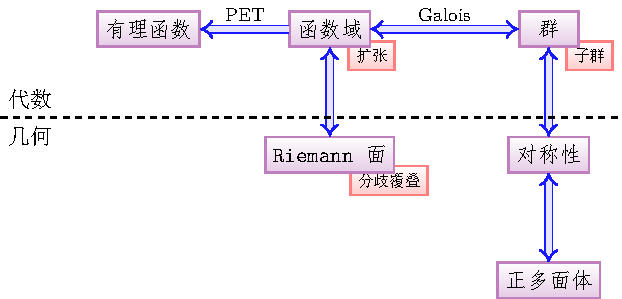
\includegraphics[]{Flowchart/flowchart1.pdf}
	\begin{minipage}[t]{.75\textwidth}
	\vspace{-2cm}
	\begin{theorem}[本原元定理(PET)]
		域$\mathbb{C}(x)$的有限扩域$E$是单扩域,即,存在$y \in E$使得$E =\mathbb{C}(x)(y)$.
	\end{theorem}
	
\end{minipage}
\end{frame}
	\begin{frame}
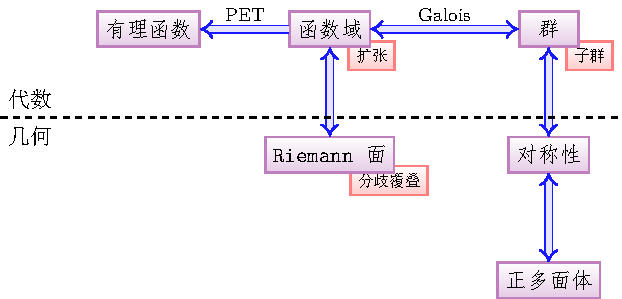
\includegraphics[]{Flowchart/flowchart1.pdf}
\begin{minipage}[t]{.75\textwidth}
	\vspace{-1cm}
	$$\varPhi:\mathbb{PC}^1\xtwoheadrightarrow{}\mathbb{PC}^1/\Gamma\overset{\sim}{\longrightarrow}\mathbb{PC}^1$$
	
\end{minipage}

\end{frame}



\begin{frame}{正十二面体群$\Gamma_{(2,3,5)} \cong A_5$}
\begin{columns}
	\begin{column}{0.7\textwidth}
		\begin{itemize}
			\item 图\ref{eg:fig1}给出$\Gamma_{(2,3,5)}$的一个12阶子群$\Gamma_{(2,3,4)}$;
			
			\item 不同的正方体给出不同且互相共轭的12阶子群;
			
			\item $\Gamma_{(2,3,5)}$中的元素给出5个正方体的置换,即群同态$$\alpha:\Gamma_{(2,3,5)}\longrightarrow S_5.$$
			易验证$\ker(\alpha)=\{Id\}$, $Im(\alpha)=A_5$.因此$\Gamma_{(2,3,5)}\cong A_5$.
			
		\end{itemize}
	\end{column}
	\begin{column}{0.3\textwidth}
		\begin{figure}[ht]
			\centering
			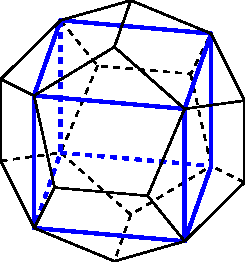
\includegraphics[scale=0.6]{poly/poly24.pdf}
			\caption{嵌套正多面体}
			\label{eg:fig1}
		\end{figure}
	\end{column}
\end{columns}
\end{frame}

	\begin{frame}{例:正十二面体}
	\hspace{-2em}
	$$\varPhi:\mathbb{PC}^1\xtwoheadrightarrow{}\mathbb{PC}^1/\Gamma\overset{\sim}{\longrightarrow}\mathbb{PC}^1$$
\begin{figure}[ht]
	
	\begin{minipage}[t]{.34\textwidth}
		\vspace{0.1cm}
		%正十二面体
		\centering
		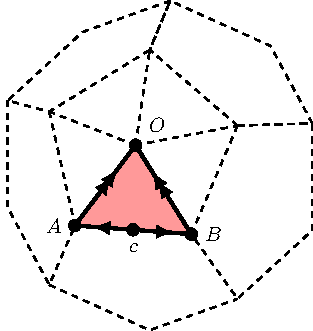
\includegraphics[width=2.25cm]{poly/poly4-2.pdf}
		
	\end{minipage}
	\begin{minipage}[t]{.64\textwidth}
		\vspace{0.1cm}
		\centering
		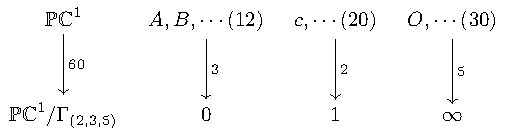
\includegraphics[scale=0.75]{commu/commu2.pdf}\\[0cm]
		在$0,1,\infty$处分歧,分歧指标为$(2,3,5)$
	\end{minipage}
	\caption{正十二面体}
	\label{pic:comm2}
\end{figure}
\end{frame}

	\begin{frame}{任务}
\hspace{-2em}
$$\varPhi:\mathbb{PC}^1\xtwoheadrightarrow{}\mathbb{PC}^1/\Gamma\overset{\sim}{\longrightarrow}\mathbb{PC}^1$$

\begin{itemize}
	\item 给出$\varPhi$的表达式;
	\item 描述$\mathbb{PC}^1/\Gamma$上的亚纯函数;
	\item<0> 描述$\varPhi^{-1}$.
\end{itemize}
\end{frame}


\subsection{不变量理论}

\begin{frame}{寻找正多面体方程的流程}
\centering
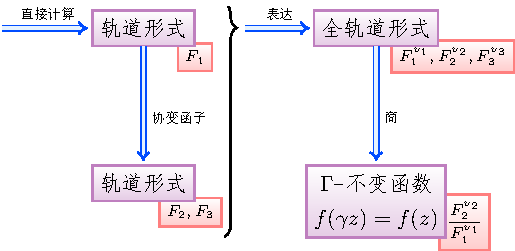
\includegraphics[scale=0.8]{Flowchart/flowchart2.pdf}
\begin{defn}[轨道形式]
	我们称轨道形式$F\in \mathbb{C}[z_1,z_2]$为满足
	$$F \circ \gamma'= \bigchi_F(\gamma') F \qquad \text{对任意$\gamma' \in \Gamma'$}$$
	的齐次多项式,其中$\bigchi_F: \Gamma' \longrightarrow \mathbb{C}^*$为某个特征.
\end{defn}
\end{frame}
\begin{frame}{正多面体方程}
	\begin{table}[ht]
	\centering
	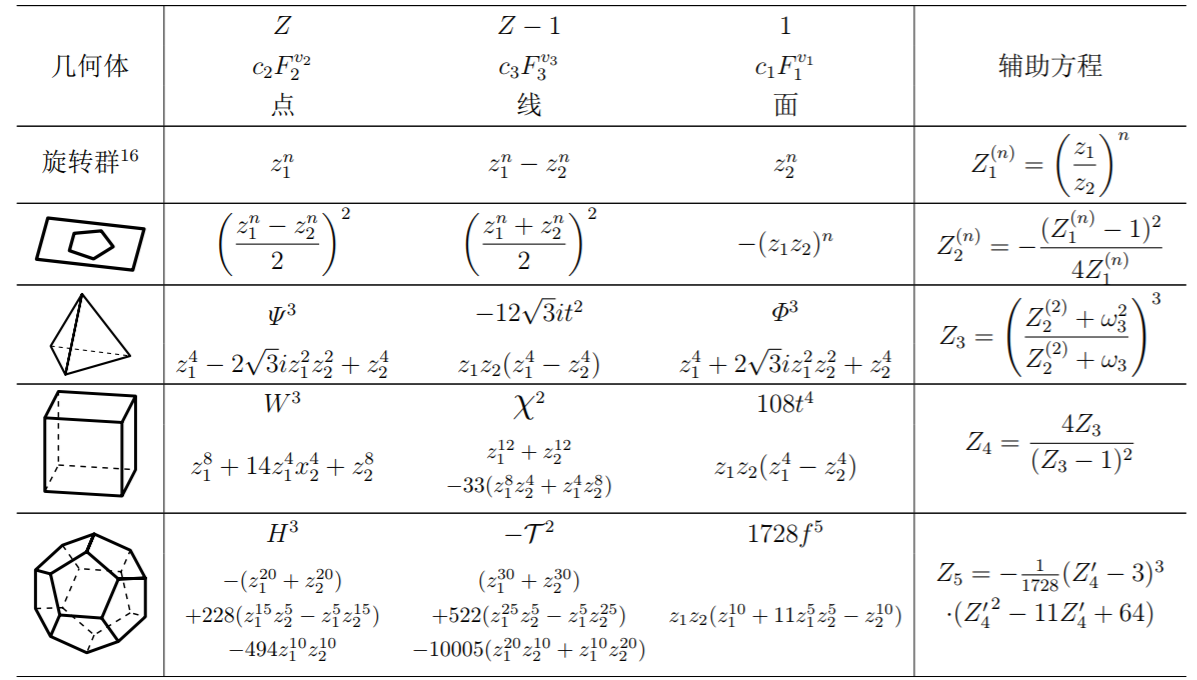
\includegraphics[width=0.9\textwidth]{snip/eqpoly.png}
	\caption{正多面体对应方程}
	\label{tb:equations}
\end{table}
\end{frame}
	\begin{frame}[<+->]{任务}
\hspace{-2em}
$$\varPhi:\mathbb{PC}^1\xtwoheadrightarrow{}\mathbb{PC}^1/\Gamma\overset{\sim}{\longrightarrow}\mathbb{PC}^1$$
对于正十二面体,
\begin{itemize}
	\item 给出$\varPhi$的表达式:
	$$\varPhi=\frac{H^{\,3}}{1728f^{\,5}}$$
	\item 描述$\mathbb{PC}^1/\Gamma$上的亚纯函数:
	$$\mathcal{M}(\mathbb{PC}^1/\Gamma)=\mathbb{C}(\varPhi)$$
	\item 描述$\varPhi^{-1}$.
\end{itemize}
\end{frame}
	\begin{frame}{任务}
$$\varPhi:\mathbb{PC}^1\xtwoheadrightarrow{}\mathbb{PC}^1/\Gamma\overset{\sim}{\longrightarrow}\mathbb{PC}^1$$
\begin{itemize}
	\item 给出$\varPhi$的表达式;
	\item 描述$\mathbb{PC}^1/\Gamma$上的亚纯函数;
	\item 描述$\varPhi^{-1}$.
	\begin{itemize}
		\item\alert<1>{复分析视角:多值函数;}
		\item<0> 近世代数视角:预解式.
	\end{itemize}
\end{itemize}
\end{frame}
\subsection{复分析视角:多值函数}
	\begin{frame}{多值函数}
	$$\hspace{-2.5cm}\varPhi^{-1}\colon\hspace{1cm} \mathbb{PC}^1/\Gamma\hspace{2cm} \longrightarrow \hspace{2cm}\mathbb{PC}^1$$
	\begin{figure}[ht]
	\centering
	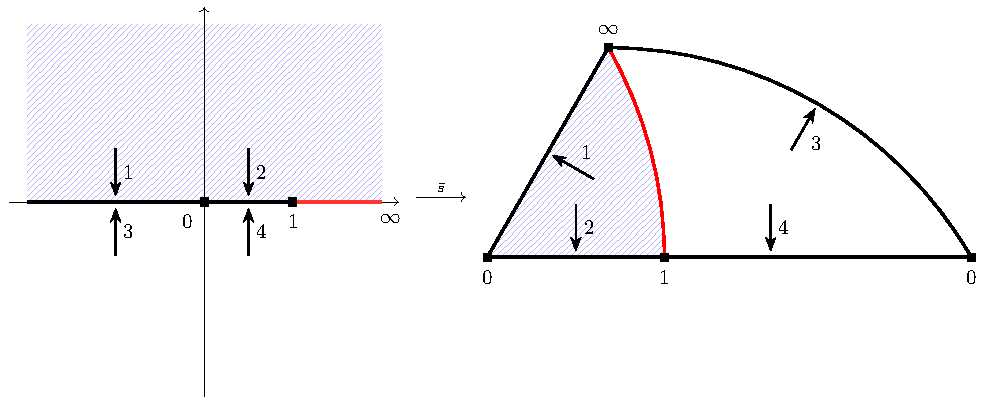
\includegraphics[width=.98\textwidth]{pic/halfspace4.pdf}
	\label{pic:Ctriangle}
\end{figure}
\end{frame}
	\begin{frame}{不同多面体对应图像:正八面体}
%%等待拍照???
\end{frame}
	\begin{frame}{不同多面体对应图像:正十二面体}
%%等待拍照???
\end{frame}
	\begin{frame}{接下来的相关工作}
我们可以得到
\begin{itemize}[<+->]
	\item 单值解析分支的表达式;
	\item 不同单值解析分支之间的关系;
	\item 单值解析分支满足的常微分方程.
\end{itemize}
\end{frame}
\section{五次方程的解}
\begin{frame}{流程图}
	\begin{columns}
		\begin{column}{0.4\textwidth}
		\begin{figure}[ht]
			\centering
			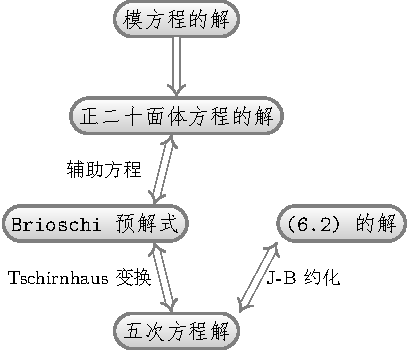
\includegraphics[scale=0.7]{Flowchart/Mainflowchart-1.pdf}
		\end{figure}
	\end{column}
	\begin{column}{0.6\textwidth}
	\begin{figure}[ht]
		\centering
		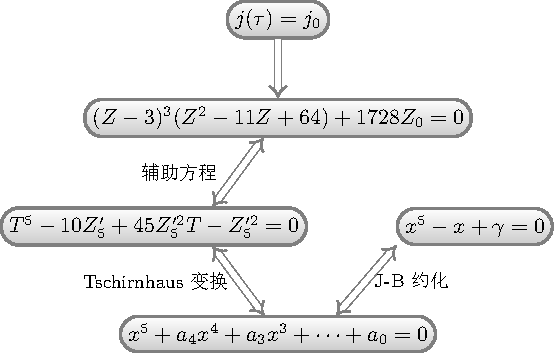
\includegraphics[scale=0.7]{Flowchart/Mainflowchart-2.pdf}
	\end{figure}
\end{column}
	\end{columns}
\end{frame}
	\begin{frame}{预解式}
时间关系跳过。。。
\end{frame}
	\begin{frame}[fragile]{模方程解正二十面体方程}
$$\text{记 \;}\Gamma(N):=\left\{ \begin{pmatrix}
a &b \\ c & d
\end{pmatrix} \in SL_2(\mathbb{Z}) \;\middle|\; \begin{pmatrix}
a &b \\ c & d
\end{pmatrix} \equiv \begin{pmatrix}
1 &0 \\ 0 & 1
\end{pmatrix} \mod N  \right\}$$
则有交换图

\begin{center}
	\begin{tikzcd}
	\mathcal{H}^* \arrow[r, "r"] & \mathcal{H}^*/\Gamma(5) \arrow[r, "\pi_1"] \arrow[d, "\hat{j}_5","\sim"'] & \mathcal{H}^*/\Gamma(1) \arrow[d, "\hat{j}","\sim"'] \\
	& \mathbb{PC}^1 \arrow[r, "I"]                                      & \mathbb{PC}^1                               
\end{tikzcd}
\end{center}

\end{frame}
\section{模空间与$\theta$函数}
	\begin{frame}{$\mathbb{C}/\Lambda$与$\mathcal{H}/SL_2(\mathbb{Z})$}
\begin{table}[ht]
	\centering
	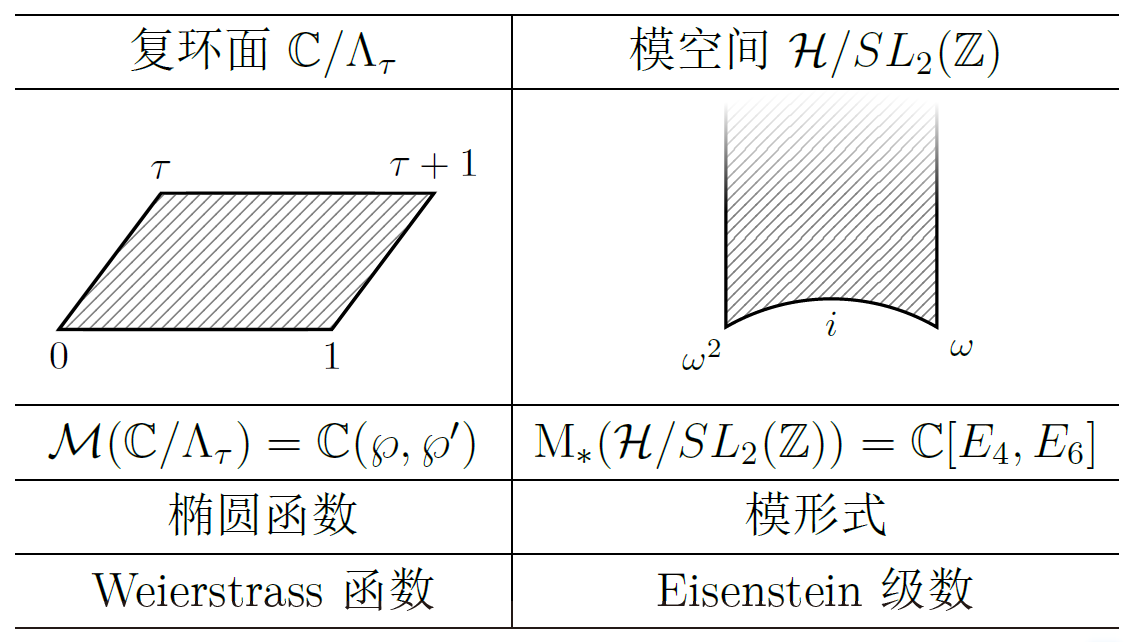
\includegraphics[width=0.8\textwidth]{snip/table-torus-moduli.png}
	\caption{复环面与模空间的比较}
	\label{tb:torus-moduli}
\end{table}
\end{frame}
\begin{frame}{$\mathcal{H}/\Gamma(N)$}
%%插入N=5,N=7的图片
\end{frame}
\begin{frame}{$\mathcal{H}/\Gamma(N)$上的"函数":$\theta$-函数}
\begin{defn}
	我们定义带特征$\chi:=\normalcharacter \in \mathbb{R}^2$的$\theta$-函数
	$$\theta\normalcharacter : 
	\mathbb{C} \times \mathcal{H} \longrightarrow \mathbb{C}$$
	$$\theta\normalcharacter(z, \tau)=\sum_{n \in \mathbb{Z}} \exp 2 \pi i \left\{\frac{1}{2}\left(n+\frac{\epsilon}{2}\right)^{2} \tau+\left(n+\frac{\epsilon}{2}\right)\left(z+\frac{\epsilon^{\prime}}{2}\right)\right\}$$
	
	注意到$\theta$-函数的良定性,且分别关于$z$, $\tau$全纯.
\end{defn}
\end{frame}
\begin{frame}{$\theta$-函数的意义}
%本节跳过
\begin{table}[ht]
	\centering
	
\includegraphics[width=0.8\textwidth]{snip/table-geomean.png}
	\caption{参数所代表的几何意义}
\end{table}
\end{frame}
\begin{frame}{$\theta$-函数的结论}
\begin{theorem}[{\cite[p218]{farkas2001theta}}]
	设$N$为奇素数,对$l=0,\ldots,\frac{N-3}{2}$,取$\chi_l:= \character{\frac{2l+1}{N}}{1}$,定义全纯函数
	$$\varphi_l: \mathcal{H} \longrightarrow \mathbb{C} \qquad \tau \longmapsto \theta[\chi_l](0,N\tau)$$
	则$\varphi_l$为级$\Gamma(N)$权$1/2$的模形式,且具有相同特征$\bigchi_k$.
	<2->
	通俗地说,对任意$\gamma=\begin{pmatrix}
	a & b\\c & d
	\end{pmatrix} \in \Gamma(N)$,函数$\varphi_l$均满足等式
	$$\varphi_l(\gamma z)= \bigchi_k(\gamma) (cz+d)^{\frac{1}{2}} \varphi_l(z)$$
\end{theorem}

\end{frame}
\begin{frame}{亚纯函数与射影嵌入}
\begin{theorem}
	对$N=5,7$, $\varphi_l/\varphi_{l^{\,'}}$为$\mathcal{H}^{*}/\Gamma(N)$上的亚纯函数,且我们有射影嵌入
$$\Phi: \mathcal{H}^*/\Gamma(N) \longrightarrow \mathbb{PC}^{\frac{N-3}{2}} \qquad \bar{\tau} \longmapsto \left[ \varphi_0(\tau),\ldots , \varphi_{\frac{N-3}{2}}(\tau) \right]$$
\end{theorem}
\end{frame}
\subsection{应用}
\begin{frame}{$N=5$}

	我们有同构(记$\hat{j}_5:=\varPhi$)
	$$\hat{j}_5: \mathcal{H}^*/\Gamma(5) \longrightarrow \mathbb{PC}^{1} \qquad \bar{\tau} \longmapsto \left[ \varphi_0(\tau),\varphi_{1}(\tau) \right]$$
并且$\hat{j}_5$将$\Gamma(1)\infty$映至正十二面体的12个面心顶点上,将$\Gamma(1)i$映至边点,将$\Gamma(1)\omega_3$映至顶点上。这给出了我们之前需要的性质。
\end{frame}
\begin{frame}{$N=7$}

	我们有射影嵌入
	$$\varPhi: \mathcal{H}^*/\Gamma(7) \longrightarrow \mathbb{PC}^{1} \qquad \bar{\tau} \longmapsto \left[ \omega_7^4\varphi_0(\tau),\varphi_{1}(\tau),\varphi_{2}(\tau) \right]$$
	满足方程
	$$X^3Y+Y^3Z+Z^3X=0$$
	故$\mathcal{H}^*/\Gamma(7) \cong \Proj\mathbb{C}[X,Y,Z]/(X^3Y+Y^3Z+Z^3X)$,称为Klein四次曲线。
	
	Klein四次曲线还有其它的表达,比如射影曲线$Y^7=X^2(X-1)$.它的对称性值得一提。
\end{frame}
%%%%%%%%%%%%%%%%%%%%%%%%%%%%%%%%%%%%%%%%%%%%%%%%%%%%%%%%%%%%%%%%%%%%%%%%%%




%%%%%%%%%%%%%%%%%%%%%%%%%%%%%%%%%%%%%%%%%%%%%%%%%%%%%%%%%%%%%%%%%%%%%%%%%%%%%%%%%%%%%%%%%%%%%%%







\end{document}




